\documentclass[numbers=enddot,12pt,final,onecolumn,notitlepage]{scrartcl}%
\usepackage[paperwidth=21cm,paperheight=500cm,margin=1in]{geometry}
\usepackage{amsmath}
\usepackage{amssymb}
\usepackage{array}
\usepackage{setspace}
\usepackage{graphicx}
\usepackage{etex}
\usepackage{amsthm}
\usepackage{color}
\usepackage{wasysym}
\usepackage[all]{xy}
\usepackage{textpos}
%\usepackage{ytableau}
\usepackage{stmaryrd}
\usepackage{url}
\usepackage{color}
\usepackage{epsfig,amsfonts,mathrsfs}
\usepackage{verbatim}
\usepackage{xparse}
\usepackage{amsfonts}
\usepackage{tcolorbox}
\usepackage{hyperref}%
\setcounter{MaxMatrixCols}{30}
%TCIDATA{OutputFilter=latex2.dll}
%TCIDATA{Version=5.50.0.2960}
%TCIDATA{LastRevised=Wednesday, July 08, 2020 00:42:26}
%TCIDATA{<META NAME="GraphicsSave" CONTENT="32">}
%TCIDATA{<META NAME="SaveForMode" CONTENT="1">}
%TCIDATA{BibliographyScheme=Manual}
%BeginMSIPreambleData
\providecommand{\U}[1]{\protect\rule{.1in}{.1in}}
%EndMSIPreambleData
\definecolor{grau}{rgb}{.5 , .5 , .5}
\definecolor{dunkelgrau}{rgb}{.35 , .35 , .35}
\definecolor{schwarz}{rgb}{0 , 0 , 0}
\definecolor{violet}{RGB}{143,0,255}
\definecolor{forestgreen}{RGB}{34, 100, 34}

\newcommand{\ssty}{\scriptstyle}
\newcommand{\w}{\omega}
\newcommand{\sr}{\stackrel}
\newcommand{\ov}{\overline}
\newcommand{\ga}{\gamma}
\newcommand{\al}{\alpha}
\newcommand{\be}{\beta}
\newcommand{\si}{\sigma}
\newcommand{\la}{\lambda}
\newcommand{\eps}{\varepsilon}
\newcommand{\CC}{\mathbb{C}} % complex numbers
\newcommand{\RR}{\mathbb{R}} % real numbers
\newcommand{\QQ}{\mathbb{Q}} % rational numbers
\newcommand{\NN}{\mathbb{N}} % nonnegative integers
\newcommand{\PP}{\mathbb{P}} % positive integers
\newcommand{\ZZ}{\mathbb{Z}} % integers
\newcommand{\id}{\operatorname{id}} % identity map
\newcommand{\kk}{\mathbf{k}} % our base ring
\newcommand{\QSym}{\operatorname{QSym}}
\newcommand{\Des}{\operatorname{Des}}
\newcommand{\Odd}{\operatorname{Odd}}
\newcommand{\Comp}{\operatorname{Comp}}
\newcommand{\Peak}{\operatorname{Peak}}

% For shuffle product symbol
\makeatletter
\providecommand*{\shuffle}{%
  \mathbin{\mathpalette\shuffle@{}}%
}
\newcommand*{\shuffle@}[2]{%
  % #1: math style
  % #2: unused
  \sbox0{$#1\vcenter{}$}%
  \kern .15\ht0 % side bearing
  \rlap{\vrule height .25\ht0 depth 0pt width 2.5\ht0}%
  \raise.1\ht0\hbox to 2.5\ht0{%
    \vrule height 1.75\ht0 depth -.1\ht0 width .17\ht0 %
    \hfill
    \vrule height 1.75\ht0 depth -.1\ht0 width .17\ht0 %
    \hfill
    \vrule height 1.75\ht0 depth -.1\ht0 width .17\ht0 %
  }%
  \kern .15\ht0 % side bearing
}

\makeatother


\newcommand{\red}{\color{red}}
\newcommand{\grey}{\color{grau}}
\newcommand{\green}{\color{forestgreen}}
\newcommand{\violet}{\color{violet}}
\newcommand{\blue}{\color{blue}}
\newcommand{\EE}{{\mathbf{E}}}
\newcommand{\OO}{\operatorname {O}}
\newcommand{\Nm}{\operatorname {N}}
\newcommand{\Par}{\operatorname{Par}}
\newcommand{\Stab}{\operatorname {Stab}}
\newcommand{\ev}{\operatorname{ev}}
\newcommand{\Sym}{\operatorname{Sym}}
\newcommand{\des}{\operatorname{des}}
\newcommand{\inv}{\operatorname{inv}}
\newcommand{\maj}{\operatorname{maj}}
\newcommand{\NSym}{\operatorname{NSym}}
\newcommand{\Gr}{\operatorname{Gr}}
\newcommand{\QHo}{\operatorname{QH}}
\newcommand{\Ho}{\operatorname{H}}
\newcommand{\Mat}{\operatorname{M}}
\newcommand{\bk}{\mathbf{k}}
\newcommand{\Nplus}{\mathbb{N}_{+}}
\newcommand\arxiv[1]{\href{http://www.arxiv.org/abs/#1}{\texttt{arXiv:#1}}}
\newcommand{\GL}{\operatorname {GL}}
\newcommand{\SL}{\operatorname {SL}}
\newcommand{\Or}{\operatorname {O}}
\newcommand{\im}{\operatorname {Im}}
\newcommand{\Iso}{\operatorname {Iso}}
\newcommand{\Adm}{\operatorname{Adm}}
\newcommand{\Supp}{\operatorname{Supp}}
\newcommand{\Powser}{\QQ\left[\left[x_1,x_2,x_3,\ldots\right]\right]}
\newcommand{\rad}{\operatorname {rad}}
\newcommand{\zero}{\mathbf{0}}
\newcommand{\xx}{\mathbf{x}}
\newcommand{\ord}{\operatorname*{ord}}
\newcommand{\bbK}{{\mathbb{K}}}
\newcommand{\whP}{{\widehat{P}}}
\newcommand{\calP}{\mathcal{P}}
\newcommand{\calS}{\mathcal{S}}
\newcommand{\calI}{\mathcal{I}}
\newcommand{\rato}{\dashrightarrow}
\newcommand{\lcm}{\operatorname*{lcm}}
\newcommand{\lm}{\lambda / \mu}
\newcommand{\fti}[1]{\subsection{#1}}
\newenvironment{iframe}[1][]{ \fti{[#1]} \begin{itemize}}{\end{itemize}}
\newcommand{\are}{\ar@{-}}
\newcommand{\arinj}{\ar@{_{(}->}}
\newcommand{\arsurj}{\ar@{->>}}
\newcommand{\set}[1]{\left\{ #1 \right\}}
\newcommand{\abs}[1]{\left| #1 \right|}
\newcommand{\tup}[1]{\left( #1 \right)}
\newcommand{\ive}[1]{\left[ #1 \right]}
\newcommand{\verts}[1]{\operatorname{V}\left( #1 \right)}
\newcommand{\edges}[1]{\operatorname{E}\left( #1 \right)}
\newcommand{\arcs}[1]{\operatorname{A}\left( #1 \right)}
\newcommand{\underbrack}[2]{\underbrace{#1}_{\substack{#2}}}
\definecolor{darkred}{rgb}{0.7,0,0}
\newcommand{\defn}[1]{{\color{darkred}\emph{#1}}}
\newcommand{\defnm}[1]{{\color{darkred} #1}}
\newcommand{\STRUT}{\vrule width 0pt depth 8pt height 0pt}
\newcommand{\ASTRUT}{\vrule width 0pt depth 0pt height 11pt}
\newcommand{\iso}{\cong}
\newcommand{\fs}{\mathcal{S}}
\newcommand{\mbf}{\mathbf}
\newcommand{\0}{\phantom{c}}
\newcommand{\swt}[1]{\left\langle #1 \right\rangle}
\newcommand{\SymGp}[1]{\mathfrak{S}_{#1}}
\DeclareMathOperator{\wt}{wt}
\newcommand{\wtg}{\widetilde{g}}
\newcommand{\cont}{\operatorname{cont}}
\newcommand{\ircont}{\operatorname{ircont}}
\newcommand{\ceq}{\operatorname{ceq}}
\newcommand{\ttt}{{\mathbf{t}}}
\newcommand{\mm}{\mathbf{m}}
\newcommand{\nn}{\mathbf{n}}
\newcommand{\qq}{\mathbf{q}}
\newcommand{\mcA}{\mathcal{A}}
\newcommand{\mcF}{\mathcal{F}}
\newcommand{\mcM}{\mathcal{M}}
\newcommand{\mcW}{\mathcal{W}}
\newcommand{\mcI}{\mathcal{I}}
\let\sumnonlimits\sum
\let\prodnonlimits\prod
\let\cupnonlimits\bigcup
\let\capnonlimits\bigcap
\renewcommand{\sum}{\sumnonlimits\limits}
\renewcommand{\prod}{\prodnonlimits\limits}
\renewcommand{\bigcup}{\cupnonlimits\limits}
\renewcommand{\bigcap}{\capnonlimits\limits}
\renewcommand{\labelitemii}{$\spadesuit$}
\newcommand{\nowbox}{\hphantom{x} \vspace{-1.5pc}}

\tcbuselibrary{theorems}
\newtcbtheorem
  []% init options
  {definition}% name
  {Definition}% title
  {%
    colback=green!5,
    colframe=green!35!black,
    fonttitle=\bfseries,
  }% options
  {def}% prefix

\newtcbtheorem
  []% init options
  {theorem}% name
  {Theorem}% title
  {%
    colback=blue!5,
    colframe=blue!35!black,
    fonttitle=\bfseries,
  }% options
  {def}% prefix

\newtcbtheorem
  []% init options
  {corollary}% name
  {Corollary}% title
  {%
    colback=blue!5,
    colframe=blue!35!black,
    fonttitle=\bfseries,
  }% options
  {def}% prefix

\newtcbtheorem
  []% init options
  {proposition}% name
  {Proposition}% title
  {%
    colback=blue!5,
    colframe=blue!35!black,
    fonttitle=\bfseries,
  }% options
  {def}% prefix

\newtcbtheorem
  []% init options
  {question}% name
  {Question}% title
  {%
    colback=red!5,
    colframe=red!35!black,
    fonttitle=\bfseries,
  }% options
  {def}% prefix

\newtcbtheorem
  []% init options
  {problem}% name
  {Problem}% title
  {%
    colback=red!5,
    colframe=red!35!black,
    fonttitle=\bfseries,
  }% options
  {def}% prefix

\newtcbtheorem
  []% init options
  {conjecture}% name
  {Conjecture}% title
  {%
    colback=red!5,
    colframe=red!35!black,
    fonttitle=\bfseries,
  }% options
  {def}% prefix

\iffalse
\NOEXPAND{\defn}[1]{\defn}
\NOEXPAND{\defnm}[1]{\defnm}
\fi
\begin{document}

\title{Weighted posets and the enriched monomial basis of QSym [slides]}
\author{\href{http://www.cip.ifi.lmu.de/~grinberg/}{Darij Grinberg} and Ekaterina Vassilieva}
\date{2022-01-17}
\maketitle

\subsection*{***}

\textbf{these slides: \color{red}
\url{https://www.mat.univie.ac.at/~slc/wpapers/FPSAC2021/58Grinberg.pdf}}%
\newline\textbf{paper: \color{red}
\url{https://www.mat.univie.ac.at/~slc/wpapers/FPSAC2021/58Grinberg.pdf}}%
\newline

\begin{tcolorbox}[colback=cyan!5,colframe=cyan!75!black, fonttitle=\bfseries,title=Summary of our work] Hsiao defines in \cite{Hsi07} the \textbf{monomial peak functions} $\eta_{\al}$, a new class of quasisymmetric functions indexed by \textbf{odd compositions} of $n$. They provide a monomial like basis to Stembridge's algebra of peak \cite{Ste97} and are related to Stembridge peak functions $K_\al$ through
\begin{equation*}
K_{\al} = \sum_{{\substack{\beta \in \Odd(n);\\ \Peak(\beta) \subseteq \Peak(\al)}}} \eta_{\beta}.
\end{equation*}
In the present work: 
\begin{itemize}
\item We show that monomial peaks may be extended to all integer partitions and that this extension is \textbf{a basis of QSym} as a whole. We name this new basis the \textbf{enriched monomial basis} of QSym.
\item We relate it to other bases of QSym, compute its \textbf{antipode} and \textbf{coproduct}. 
\item We introduce a new type of \textbf{weighted posets} and their generating functions as a \textbf{universal framework} to study all types of quasisymmetric functions.

\begin{center}
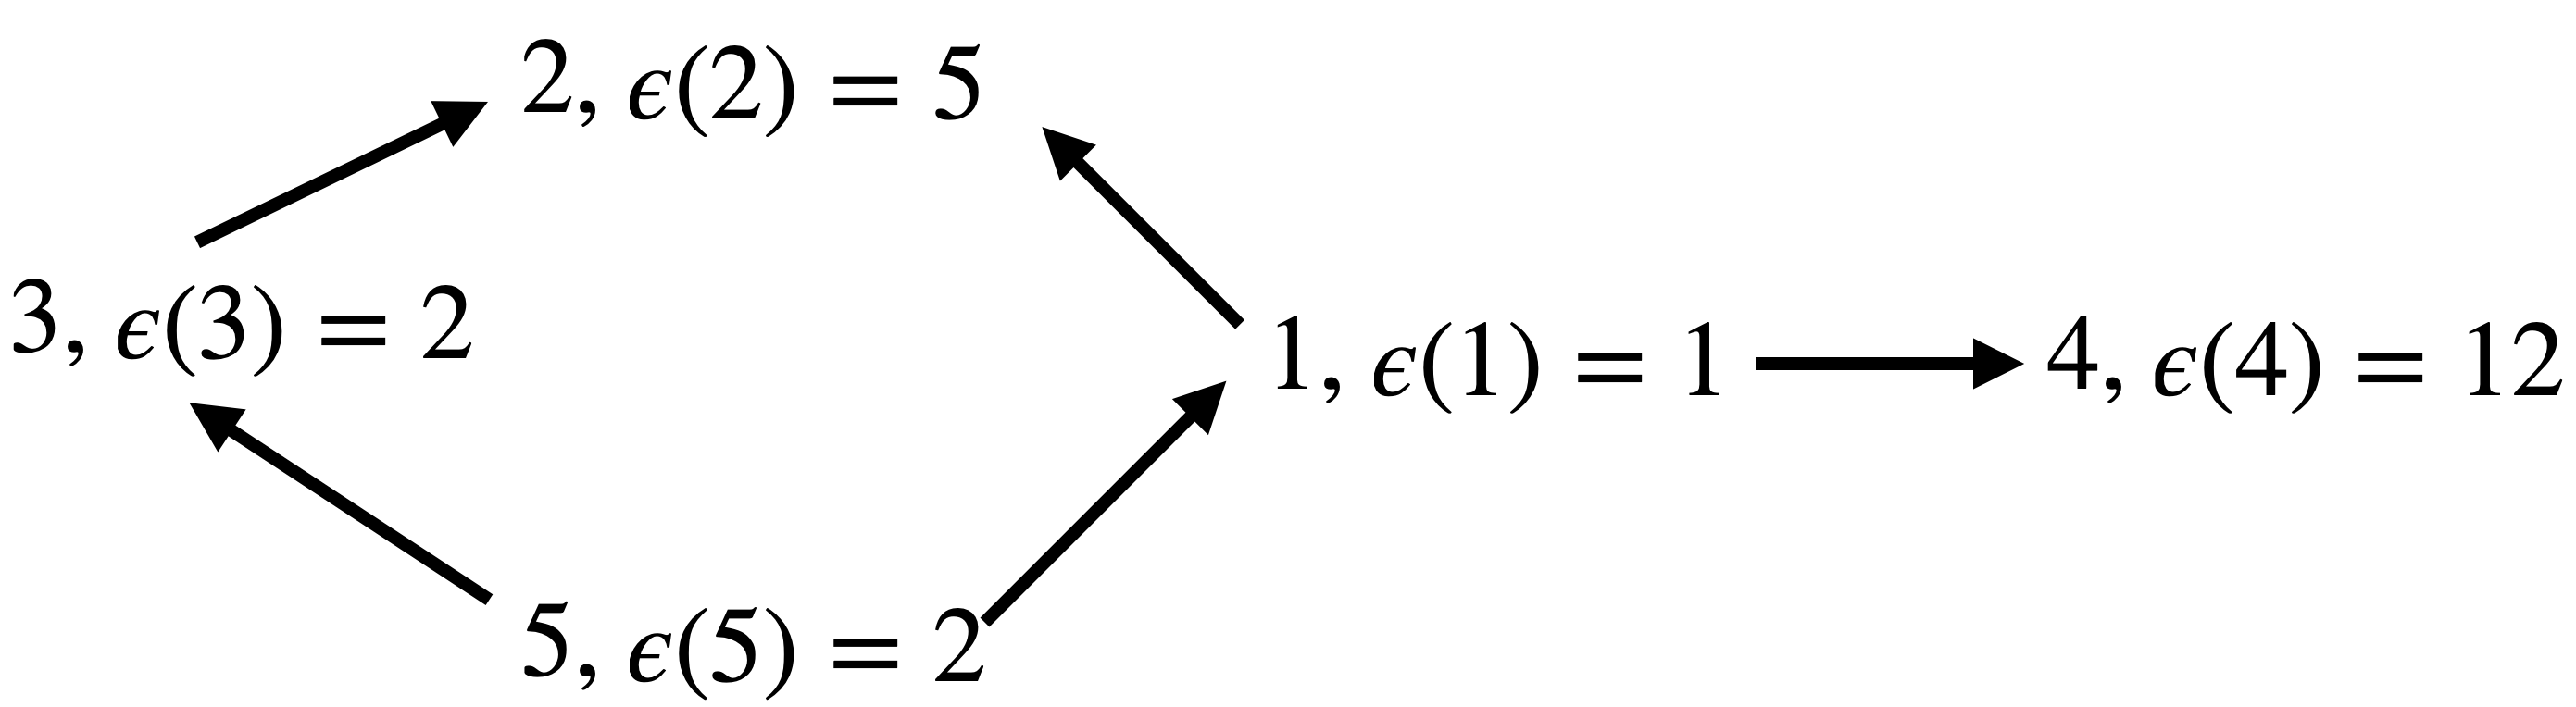
\includegraphics[scale=0.16]{Poset.png}
\end{center}
 
\item We use our framework to compute the \textbf{product} of two enriched monomials:
\begin{equation*}
\eta_\al \eta_\beta
= \sum_{\substack{\gamma \in \al \shuffle \be ;\\
                   I\subseteq \left(S_{\be}(\gamma)\setminus (S_{\be}(\gamma)-1)\right) \setminus \left\{1\right\}}}
(-1)^{|I|}\eta_{\gamma^{\downarrow\downarrow I}} .
\end{equation*}
\end{itemize}
\end{tcolorbox}

%%%%%%%%%%%%%%%%%%%%%%%%%%%%%%%%%%
%%%%%%%%%%%%%%%%%%%%%%%%%%%%%%%%%%
%%%%%%%%%%%%%%%%%%%%%%%%%%%%%%%%%%
\section{Notation and basic definitions}
%%%%%%%%%%%%%%%%%%%%%%%%%%%%%%%%%%
%%%%%%%%%%%%%%%%%%%%%%%%%%%%%%%%%%
%%%%%%%%%%%%%%%%%%%%%%%%%%%%%%%%%%


%%%%%%%%%%%%%%%%%%%%%%%%%%%%%%%%%%
\subsection{Compositions and permutations statistics}
%%%%%%%%%%%%%%%%%%%%%%%%%%%%%%%%%%

\begin{itemize}
\item $\PP =\left\{1,2,\dots\right\}$, $\NN = \left\{0,1,\ldots\right\}$, $[n] = \left\{1,2,\dots, n\right\}$, $S_n$ the symmetric group on $[n]$

\item \defn{$\Comp(n)$} is the set of \defn{compositions} $\al = (\al_1, \al_2, \dots, \al_p)$ of $n$. \defn{$\Odd(n)$} is the set of \defn{odd compositions} of $n$ containing only odd integers.  Let $\ell(\al) := p$, $|\al| := \sum_i \al_i = n$.

\item The \defn{descent set} $\Des(\pi)$ of $\pi \in S_n$ is 
$\Des(\pi) = \{1\leq i\leq n-1| \pi(i)>\pi(i+1)\}.$


\item The \defn{peak set} $\Peak(\pi)$ of $\pi$ is $
\Peak(\pi) = \{2\leq i\leq n-1| \pi(i-1)<\pi(i)>\pi(i+1)\}.$

\item Compositions of $n$ are in bijection with descent sets of permutations in $S_n$ while odd compositions of $n$, are in one-to-one correspondence with peak sets. Denote \defn{$Des(\al)$} (\defn{$Peak(\al)$}) the descent set (peak set) assiociated with  (odd) composition $\al$.

\end{itemize}

%%%%%%%%%%%%%%%%%%%%%%%%%%%%%%%%%%
\subsection{Quasisymmetric functions}
%%%%%%%%%%%%%%%%%%%%%%%%%%%%%%%%%%


\begin{itemize}
\item For any $n \in \NN$ and $\al =(\al_1,\al_2,\dots,\al_p) \in \Comp(n)$, define the \defn{monomial quasisymmetric function} $M_\al$ and the \defn{fundamental quasisymmetric function} $L_\al$ by

\begin{equation*}
\label{eq : M+L}
M_{\al} = \sum\limits_{i_1 < \cdots < i_p} x_{i_1}^{\al_1}x_{i_2}^{\al_2} \cdots x_{i_p}^{\al_p},\;\;\;\;\;\; L_{\al} = \sum\limits_{\substack{i_1 \leq \cdots \leq i_n;\\j\in \Des(\al) \Rightarrow i_j<i_{j+1}}} x_{i_1}x_{i_2} \cdots x_{i_n}.
\end{equation*}

\item As an example, for $n=3$, we have
\begin{gather*}
M_{(2,1)}=\sum_{i<j}x_{i}^{2}x_{j}=x_{1}^{2}x_{2}+x_{1}%
^{2}x_{3}+x_{2}^{2}x_{3}+x_{1}^{2}x_{4}+x_{2}^{2}x_{4}+x_{3}^{2}x_{4}+\dots,\\
L_{(2,1)}=\sum_{i\leq j <k}x_{i}x_{j}x_k=x_{1}^{2}x_{2}+x_{1}%
^{2}x_{3}+x_{1}x_{2}x_3+x_{2}^{2}x_{3}+x_{1}^{2}x_{4}+x_{1}
x_{2}x_{4}+x_{2}^{2}x_{4}+\dots.
\end{gather*}
\item The sets $\left\{M_\al\right\}_{n\in \NN,\ \al\in \Comp(n)}$
and $\left\{L_\al\right\}_{n\in \NN,\ \al\in \Comp(n)}$
are two bases of the $\kk$-module $\QSym$.
They are related through
\begin{equation}
\label{eq : LM} L_{\al} = \sum_{{\substack{\beta \in \Comp(n);\\\Des(\alpha) \subseteq \Des(\beta)}}} M_{\beta}.
\end{equation}
\end{itemize}

%%%%%%%%%%%%%%%%%%%%%%%%%%%%%%%%%%
\subsection{Peak and monomial peak functions}
%%%%%%%%%%%%%%%%%%%%%%%%%%%%%%%%%%

\begin{itemize}
\item In \cite{Ste97}, Stembridge introduces \defn{peak} quasisymmetric functions. Given $n \in \NN$ and $\al \in \Odd(n)$,
\begin{equation*}
\label{eq : K}
K_{\al} = \sum\limits_{\substack{i_1 \leq \dots \leq i_n;\\j\in \Peak(\al) \Rightarrow  i_{j-1}<i_{j+1}}}2^{|\{i_1,i_2,\dots,i_n\}|} x_{i_1}x_{i_2} \cdots x_{i_n}.
\end{equation*}
\item  Hsiao defines in \cite{Hsi07} the \defn{monomial peak functions}. For any odd composition $\al =(\al_1,\al_2,\dots,\al_p)\in \Odd(n)$, let
\begin{equation}
\label{eq : monpeak}
\eta_{\al} = (-1)^{(n-\ell(\al))/2}\sum\limits_{\substack{i_1 \leq \dots \leq i_p}}2^{|\{i_1,i_2,\dots,i_p\}|} x_{i_1}^{\al_1}x_{i_2}^{\al_2} \cdots x_{i_p}^{\al_p}.
\end{equation}
\item An identity similar to Equation (\ref{eq : LM}) relates peak and monomial peak functions:
\begin{equation}
\label{eq : KE} K_{\al} = \sum_{{\substack{\beta \in \Odd(n);\\ \Peak(\beta) \subseteq \Peak(\al)}}} \eta_{\beta}.
\end{equation}
\end{itemize}

%%%%%%%%%%%%%%%%%%%%%%%%%%%%%%%%%%
\subsection{Posets and $P$-partitions}
%%%%%%%%%%%%%%%%%%%%%%%%%%%%%%%%%%
\label{sec : poset}

\begin{itemize}
\item A \defn{labelled poset} $P=([n],<_P)$ is an arbitrary partial order $<_P$ on the set $[n]$. 
\item Let $P = ([n],<_P)$ be a labelled poset.
A \defn{$P$-partition} is a map $f: [n]\longrightarrow \PP$ that satisfies the two following conditions:
\begin{itemize}
\item[(i)] If $i <_P j$, then $f(i) \leq f(j)$.
\item[(ii)] If $i <_P j$ and $i > j$, then $f(i) < f(j)$.
\end{itemize}
\item Let $\PP^{\pm}=\left\{-,+\right\} \times \PP$. We equip the set $\PP^{\pm}$ with a total order given by $-1<1<-2<2<-3<\dots$. 
Let $P = ([n],<_P)$ be a labelled poset.
An \defn{enriched $P$-partition} is a map $f: [n]\longrightarrow \PP^{\pm} $ that satisfies the following two conditions:
\begin{itemize}
\item[(i)] If $i <_P j$ and $i < j$, then $f(i) < f(j)$ or $f(i) = f(j) \in \PP$.
\item[(ii)] If $i <_P j$ and $i>j$, then $f(i) < f(j)$ or $f(i) = f(j) \in -\PP$.
\end{itemize} 
\item A more general concept was defined in \cite{Gri18}: Let $\mathcal{Z}$ be a subset of the totally ordered set $\PP^{\pm}$ and $P=([n],<_P)$ be a labelled poset.
A \defn{$\mathcal{Z}$-enriched $P$-partition} is
an enriched $P$-partition $f : [n] \longrightarrow \PP^{\pm} $ with $f([n]) \subseteq \mathcal{Z}$.
Let $\mathcal{L}_\mathcal{Z}(P)$ denote the set of $\mathcal{Z}$-enriched $P$-partitions.

\item Let $X = \left\{x_1,x_2,x_3,\ldots\right\}$, $P =([n],<_P)$, and $\mathcal{Z} \subseteq \PP^{\pm}$. Define the  \defn{$\mathcal{Z}$-generating function of $P$} as the formal power series
\begin{align}
\label{eq : GammaTrad}
\Gamma_{\mathcal{Z}}([n], <_P) &= \sum_{f \in \mathcal{L}_\mathcal{Z}([n],<_P)}\ \ \prod_{1\leq i \leq n}x_{|f(i)|} .
\end{align}
\item Given $\pi \in S_n$, let $P_\pi = ([n],<_\pi)$ denote the labelled poset where the order relation $<_\pi$ is such that $\pi_i <_\pi \pi_j$ if and only if $i < j$ (see Figure \ref{fig : ppart}).
\begin{figure}[htbp]
\begin{center}
 \includegraphics[scale=0.20]{PPart}\caption{The labelled poset associated to permutation $\pi$.}
 \label{fig : ppart}
 \end{center}
 \end{figure}

\item Set $L_{\pi}= \Gamma_{\PP}([n],<_\pi)$ and $K_{\pi}= \Gamma_{\PP^\pm}([n],<_\pi)$. The function $L_\pi$ is equal to the fundamental quasisymmetric function $L_\al$ indexed by the unique composition $\al$ such that $\Des(\al) = \Des(\pi)$. Similarly, $K_\pi$ is equal to the peak function $K_\al$ indexed by the unique odd composition $\al$ such that $\Peak(\al) = \Peak(\pi)$. 
%\end{proposition}
%This description leads to easy product formulas for both fundamental and peak quasisymmetric functions. Indeed, one has the following proposition.
%\begin{proposition}[\cite{Ges84, Ste97}]
\item Given two permutations $\pi \in S_n$ and $\sigma \in S_m$\begin{equation}
\label{eq : GGG}
\Gamma_{\mathcal{Z}}([n],<_\pi)\Gamma_{\mathcal{Z}}([m],<_\sigma) = \sum_{\gamma \in \pi \shuffle \sigma}\Gamma_{\mathcal{Z}}([n+m],<_\gamma) .
\end{equation}
\begin{equation}
L_{\pi}L_{\sigma} = \sum_{\gamma \in \pi \shuffle \sigma}L_{\gamma}, \qquad
K_{\pi}K_{\sigma} = \sum_{\gamma \in \pi \shuffle \sigma}K_{\gamma}.
\end{equation}
\end{itemize}

\subsection{Petrie functions: definition of $G(k,m)$}

\begin{itemize}
\item \nowbox
\begin{definition}{Petrie function $G(k,m)$}{def.petGkm}
For any positive integer $k$ and any $m\in\mathbb{N}$, we let%
\begin{align*}
\defnm{G\left( k,m\right)}  &  =\sum_{\substack{\alpha\in\operatorname*{WC}%
;\\\left\vert \alpha\right\vert =m;\\\alpha_{i}<k\text{ for all }i}%
}\mathbf{x}^{\alpha}\\
&  =\sum\left(  \text{all degree-}m\text{ monomials whose exponents are all
}<k\right) \\
&  \in\Lambda.
\end{align*}
\end{definition}

For example,%
\begin{align*}
G\left(  3,4\right)   &  =\sum_{i<j<k<\ell}x_{i}x_{j}x_{k}x_{\ell}%
+\sum_{i<j<k}x_{i}^{2}x_{j}x_{k}+\sum_{i<j<k}x_{i}x_{j}^{2}x_{k}+\sum
_{i<j<k}x_{i}x_{j}x_{k}^{2}+\sum_{i<j}x_{i}^{2}x_{j}^{2}\\
&  =m_{\left(  1,1,1,1\right)  }+m_{\left(  2,1,1\right)  }+m_{\left(
2,2\right)  }.
\end{align*}

\item \textbf{Prior appearances:} $G\left(k, m\right)$ is called the
\emph{modular complete symmetric function $h'_m$} in
\begin{itemize}
\item {\red \href{https://doi.org/10.1016/0022-4049(92)90007-3}{Stephen Doty, Grant
Walker, \textit{Modular symmetric functions and irreducible modular
representations of general linear groups}, J. Pure Appl. Algebra \textbf{82}
(1992), no. 1, pp. 1--26.}}
\end{itemize}
(They keep $k$ implicit.)

\item It is also called the
\emph{truncated homogeneous symmetric function}
$h_{m}^{\left[  k-1\right]  }$
in
\begin{itemize}
\item {\red \href{https://arxiv.org/abs/2002.02784v1}{Houshan
Fu, Zhousheng Mei, \textit{Truncated Homogeneous Symmetric Functions},
arXiv:2002.02784v1}. }
\end{itemize}

\item Its version for finitely many variables also was studied (briefly) in
\begin{itemize}
\item {\red
\href{https://doi.org/10.3906/mat-1705-27}{Abdelghafour Bazeniar, Moussa Ahmia, Hac\`{e}ne
Belbachir, \textit{Connection between bi}$^{s}$\textit{nomial coefficients and
their analogs and symmetric functions}, Turk J Math \textbf{42} (2018), pp.
807--818.}}
\end{itemize}
\end{itemize}

\subsection{Petrie functions: basic properties}

\begin{itemize}
\item I named $G\left(  k\right)  $ and $G\left(  k,m\right)  $ the
\defn{Petrie functions}, for reasons that will become clear eventually.

\item \nowbox
\begin{proposition}{Basic properties of Petrie functions}{prop.basic}
Let $k > 0$ and $m \in \mathbb{N}$. Then:

\begin{itemize}
\item
\[
G\left(  k\right)  =\sum_{\substack{\lambda\in\operatorname*{Par}%
;\\\lambda_{i}<k\text{ for all }i}}m_{\lambda}=\prod_{i=1}^{\infty}\left(
x_{i}^{0}+x_{i}^{1}+\cdots+x_{i}^{k-1}\right)  .
\]


\item $G\left(  k,m\right)  $ is the $m$-th degree component of $G\left(
k\right)  $.

\item
\[
G\left(  k,m\right)  =\sum_{\substack{\lambda\in\operatorname*{Par}%
;\\\left\vert \lambda\right\vert =m;\\\lambda_{i}<k\text{ for all }%
i}}m_{\lambda}.
\]


\item $G\left(  2,m\right)  =e_{m}$.

\item $G\left(  k,m\right)  =h_{m}$ whenever $k>m$.

\item $G\left(  m,m\right)  =h_{m}-p_{m}$.
\end{itemize}
\end{proposition}

\end{itemize}

\subsection{Petrie functions and the coproduct of $\Lambda$}

\begin{itemize}
\item This is for the friends of Hopf algebras:%
\begin{proposition}{Comultiplication of Petrie functions}{prop.comul}
\[
\Delta\left(  G\left(  k,m\right)  \right)  =\sum_{i=0}^{m}G\left(
k,i\right)  \otimes G\left(  k,m-i\right)
\]
for each $k>0$ and $m\in\mathbb{N}$.
\end{proposition}

Here, \defn{$\Delta$} is the \defn{comultiplication} of $\Lambda$, defined to
be the $\mathbf{k}$-algebra homomorphism%
\begin{align*}
\Delta:\Lambda &  \rightarrow\Lambda\otimes\Lambda,\\
e_{n}  &  \mapsto\sum_{i=0}^{n}e_{i}\otimes e_{n-i}.
\end{align*}


\item In terms of alphabets, this says%
\begin{align*}
&  \left(  G\left(  k,m\right)  \right)  \left(  x_{1},x_{2},x_{3}%
,\ldots,y_{1},y_{2},y_{3},\ldots\right) \\
&  =\sum_{i=0}^{m}\left(  G\left(  k,i\right)  \right)  \left(  x_{1}%
,x_{2},x_{3},\ldots\right)  \cdot\left(  G\left(  k,m-i\right)  \right)
\left(  y_{1},y_{2},y_{3},\ldots\right)  .
\end{align*}

\end{itemize}

\subsection{Expanding Petries in the Schur basis}

\begin{itemize}
\item We can expand the $G\left(  k,m\right)  $ in the Schur basis $\left(
s_{\lambda}\right)  _{\lambda\in\operatorname*{Par}}$: e.g.,%
\[
G\left(  4,6\right)  =s_{\left(  2,1,1,1,1\right)  }-s_{\left(
2,2,1,1\right)  }+s_{\left(  3,3\right)  }.
\]


\item Surprisingly, it turns out that all coefficients are in $\left\{
0,1,-1\right\}  $.

\item Better yet: Any product $G\left(  k,m\right)  \cdot s_{\mu}$ expands in
the Schur basis with coefficients in $\left\{  0,1,-1\right\}  $.

\item Let us see what the coefficients are.
\end{itemize}

\subsection{Petrie numbers}

\begin{itemize}
\item We let $\left[  \mathcal{A}\right]  $ denote the \defn{truth value} of a
statement $\mathcal{A}$ (that is, $1$ if $\mathcal{A}$ is true, and $0$ if
$\mathcal{A}$ is false).

\item \nowbox
\begin{definition}{Petrie numbers}{def.petrienum}
Let $\lambda=\left(  \lambda_{1},\lambda_{2},\ldots,\lambda_{\ell
}\right)  \in\operatorname*{Par}$ and $\mu=\left(  \mu_{1},\mu_{2},\ldots
,\mu_{\ell}\right)  \in\operatorname*{Par}$, and let $k$ be a positive
integer. Then, the
\defn{$k$-Petrie number $\operatorname*{pet}\nolimits_{k}\left(  \lambda,\mu\right)  $}
of $\lambda$ and $\mu$ is the integer defined by%
\[
\operatorname*{pet}\nolimits_{k}\left(  \lambda,\mu\right)  =\det\left(
\left(  \left[  0\leq\lambda_{i}-\mu_{j}-i+j<k\right]  \right)  _{1\leq
i\leq\ell,\ 1\leq j\leq\ell}\right)  .
\]
\end{definition}

For example, for $\ell=3$, we have%
\begin{align*}
&  \operatorname*{pet}\nolimits_{k}\left(  \lambda,\mu\right) \\
&  =\det
\left( \begin{array} [c]{ccc}\left[ 0\leq\lambda_{1}-\mu_{1}<k\right] & \left[ 0\leq\lambda_{1}-\mu _{2}+1<k\right] & \left[ 0\leq\lambda_{1}-\mu_{3}+2<k\right] \\ \left[ 0\leq\lambda_{2}-\mu_{1}-1<k\right] & \left[ 0\leq\lambda_{2}-\mu_{2}<k\right] & \left[ 0\leq\lambda_{2}-\mu_{3}+1<k\right] \\ \left[ 0\leq\lambda_{3}-\mu_{1}-2<k\right] & \left[ 0\leq\lambda_{3}-\mu_{2}-1<k\right] & \left[ 0\leq\lambda_{3}-\mu_{3}<k\right] \end{array} \right)
.
\end{align*}
For example,%
\[
\operatorname*{pet}\nolimits_{4}\left(  \left(  3,1,1\right)  ,\left(
2,1\right)  \right)  =\det\left(
\begin{array}
[c]{ccc}%
1 & 1 & 0\\
0 & 1 & 1\\
0 & 0 & 1
\end{array}
\right)  =1.
\]

\item \nowbox
\begin{proposition}{Petrie numbers can only be $0$, $1$ or $-1$}{prop.01-1}
We have $\operatorname*{pet}\nolimits_{k}\left(
\lambda,\mu\right)  \in\left\{  0,1,-1\right\}  $ for all $\lambda$ and $\mu$.
\end{proposition}

\item \textit{Proof idea.} Each row of the matrix $\left(  \left[
0\leq\lambda_{i}-\mu_{j}-i+j<k\right]  \right)  _{1\leq i\leq\ell,\ 1\leq
j\leq\ell}$ has the form
\[
(\underbrace{0,0,\ldots,0}_{a\text{ zeroes}},\underbrace{1,1,\ldots
,1}_{b\text{ ones}},\underbrace{0,0,\ldots,0}_{c\text{ zeroes}}%
)\ \ \ \ \ \ \text{for some }a,b,c\in\mathbb{N}.
\]
Thus, this matrix is the transpose of a \defn{Petrie
matrix}. Hence, its determinant is $\in\left\{  -1,0,1\right\}  $ (by
{\color{red}{\href{https://projecteuclid.org/euclid.pjm/1102912464}{Gordon and Wilkinson
1974}}}).
\end{itemize}

\subsection{Expanding Petries in the Schur basis: the formula}

\begin{itemize}
\item \nowbox
\begin{theorem}{Petrie times Schur in Schur basis}{thm.petschur}
Let $k$ be a positive integer. Let $\mu\in
\operatorname*{Par}$. Then,%
\[
G\left(  k\right)  \cdot s_{\mu}=\sum_{\lambda\in\operatorname*{Par}%
}\operatorname*{pet}\nolimits_{k}\left(  \lambda,\mu\right)  s_{\lambda}.
\]
Thus, for each $m\in\mathbb{N}$, we have%
\[
G\left(  k,m\right)  \cdot s_{\mu}
=
\sum_{\substack{\lambda\in\Par;\\ \left|\lambda\right| =
m+\left\vert \mu\right\vert}}
\operatorname*{pet}\nolimits_{k}%
\left(  \lambda,\mu\right)  s_{\lambda}.
\]
\end{theorem}

\item \nowbox
\begin{corollary}{Petrie expanded in Schur basis (also Fu/Mei)}{thm.pet-exp}
Let $k$ be a positive integer. Then,%
\[
G\left(  k\right)  =\sum_{\lambda\in\operatorname*{Par}}\operatorname*{pet}%
\nolimits_{k}\left(  \lambda,\varnothing\right)  s_{\lambda}.
\]
Thus, for each $m\in\mathbb{N}$, we have%
\[
G\left(  k,m\right)  =
\sum_{\substack{\lambda\in\Par;\\ \left|\lambda\right| = m}}
\operatorname*{pet}\nolimits_{k}\left(  \lambda,\varnothing\right)
s_{\lambda}.
\]
\end{corollary}

\item
One proof of the Theorem uses alternants; the other uses the \textquotedblleft
semi-skew Cauchy identity\textquotedblright%
\begin{align*}
\sum_{\lambda\in\operatorname*{Par}}s_{\lambda}\left(  \mathbf{x}\right)
s_{\lambda/\mu}\left(  \mathbf{y}\right)   &  =s_{\mu}\left(  \mathbf{x}%
\right)  \cdot\prod_{i,j=1}^{\infty}\left(  1-x_{i}y_{j}\right)  ^{-1}
  =s_{\mu}\left(  \mathbf{x}\right)  \cdot\sum_{\lambda\in\operatorname*{Par}%
}h_{\lambda}\left(  \mathbf{x}\right)  m_{\lambda}\left(  \mathbf{y}\right)
\end{align*}
(for any $\mu\in\operatorname*{Par}$ and for two sets of indeterminates
$\mathbf{x}=\left(  x_{1},x_{2},x_{3},\ldots\right)  $ and $\mathbf{y}=\left(
y_{1},y_{2},y_{3},\ldots\right)  $).
\end{itemize}

\subsection{What are the Petrie numbers?}

\begin{itemize}
\item We have shown that $\operatorname*{pet}\nolimits_{k}\left(  \lambda
,\mu\right)  \in\left\{  0,1,-1\right\}  $, but what exactly is it?

\item
{\color{red}{\href{https://projecteuclid.org/euclid.pjm/1102912464}{Gordon and Wilkinson
1974}}} prove that Petrie matrices have determinants $\in\left\{
0,1,-1\right\}  $ by induction. This is little help to us.
\end{itemize}

\subsection{What are the Petrie numbers? The easy case}

\begin{itemize}
\item \nowbox
\begin{proposition}{When Petrie numbers are 0}{prop.pet0}
Let $\lambda\in\operatorname*{Par}$ and $k>0$ be
such that $\lambda_{1}\geq k$. Then, $\operatorname*{pet}\nolimits_{k}\left(
\lambda,\varnothing\right)  =0$.
\end{proposition}

\item To get a description in all other cases, recall the definition of \defn{transpose (aka conjugate) partitions}:

Given a partition $\lambda\in\operatorname*{Par}$, we define the
\defn{transpose partition $\lambda^t$} of $\lambda$ to be the partition $\mu$
given by%
\[
\mu_{i}=\left\vert \left\{  j\in\left\{  1,2,3,\ldots\right\}  \ \mid
\ \lambda_{j}\geq i\right\}  \right\vert \ \ \ \ \ \ \ \ \ \ \text{for all
}i\geq1.
\]


In terms of Young diagrams, this is just flipping the diagram of $\lambda$
across the diagonal.
\end{itemize}

\subsection{What are the Petrie numbers? Formula for $\operatorname{pet}%
_{k}\left(  \lambda,\varnothing\right)  $}

\begin{itemize}
\item \nowbox
\begin{theorem}{Petrie numbers for straight shapes: explicit formula (cf. Fu/Mei)}{thm.pet-str}
Let $\lambda\in\operatorname*{Par}$ and $k>0$ be such
that $\lambda_{1}<k$. Let $\mu=\lambda^{t}$ (the transpose partition of
$\lambda$). Thus, $\mu_{k}=0$.

For each $i\in\left\{  1,2,\ldots,k-1\right\}  $, set
\[
\beta_{i}=\mu_{i}-i\qquad\text{and}\qquad\gamma_{i}=1+\underbrace{\left(
\beta_{i}-1\right)  \%k}_{\substack{\text{remainder of }\beta_{i}%
-1\\\text{modulo }k}}.
\]

\begin{itemize}

\item If the $k-1$ numbers $\gamma_{1},\gamma_{2},\ldots,\gamma_{k-1}$
are not distinct, then
\[
\operatorname*{pet}\nolimits_{k}\left(  \lambda
,\varnothing\right)  =0 .
\]

\item If the $k-1$ numbers $\gamma_{1},\gamma_{2},\ldots,\gamma_{k-1}$
are distinct, then%
\[
\operatorname*{pet}\nolimits_{k}\left(  \lambda,\varnothing\right)  =\left(
-1\right)  ^{\left(  \beta_{1}+\beta_{2}+\cdots+\beta_{k-1}\right)  +g+\left(
\gamma_{1}+\gamma_{2}+\cdots+\gamma_{k-1}\right)  },
\]
where%
\[
g=\left\vert \left\{  \left(  i,j\right)  \in\left\{  1,2,\ldots,k-1\right\}
^{2}\ \mid\ i<j\text{ and }\gamma_{i}<\gamma_{j}\right\}  \right\vert .
\]
\end{itemize}
\end{theorem}


\item \nowbox
\begin{question}{Petrie numbers: explicit formula in general?}{}
Is there such a description for $\operatorname*{pet}%
\nolimits_{k}\left(  \lambda,\mu\right)  $ ?
\end{question}
\end{itemize}

\subsection{Other properties}

\begin{itemize}
\item For any $k>0$, we define a map $\defnm{\mathbf{f}_{k}}:\Lambda
\rightarrow\Lambda$ by setting%
\[
\mathbf{f}_{k}\left(  a\right)  =a\left(  x_{1}^{k},x_{2}^{k},x_{3}^{k}%
,\ldots\right)  \ \ \ \ \ \ \ \ \ \ \text{for each }a\in\Lambda.
\]
This map $\mathbf{f}_{k}$ is called the \defn{$k$-th Frobenius endomorphism}
of $\Lambda$. (Also known as plethysm by $p_{k}$. Perhaps the nicest plethysm!)

\item \nowbox
\begin{theorem}{Petrie functions in terms of $h$, $e$ and Frobenius}{thm.frob}
Let $k$ be a positive integer. Let $m\in\mathbb{N}$.
Then,%
\[
G\left(  k,m\right)  =\sum_{i\in\mathbb{N}}\left(  -1\right)  ^{i}%
h_{m-ki}\cdot\mathbf{f}_{k}\left(  e_{i}\right)  .
\]
\end{theorem}

\item \nowbox
\begin{theorem}{Petrie functions as basis (Doty/Walker)}{thm.petrie-basis}
Fix a positive integer $k$. Assume that $1-k$ is
invertible in $\mathbf{k}$. Then, the family
\[
\left(  G\left(  k,m\right)
\right)  _{m\geq1}=\left(  G\left(  k,1\right)  ,G\left(  k,2\right)
,G\left(  k,3\right)  ,\ldots\right)
\]
is an algebraically independent
generating set of the commutative $\mathbf{k}$-algebra $\Lambda$.
\end{theorem}

\item Thus, products of several elements of this family form a basis of
$\Lambda$ (if $1-k$ is invertible in $\mathbf{k}$). These bases remain to be studied.
\end{itemize}

\subsection{A conjecture of Alexandersson}

\begin{itemize}

\item \nowbox
\begin{conjecture}{(Per Alexandersson, 2020)}{}
Let $k$ be a positive integer, and $m\in\mathbb{N}$. Then,
$G\left(  k,m\right)  \cdot p_{2}\in\Lambda$ can be written in the form
$\sum_{\lambda\in\operatorname*{Par}}u_{\lambda}s_{\lambda}$ with $u_{\lambda
}\in\left\{  -1,0,1\right\}  $ for all $\lambda\in\operatorname*{Par}$.
\end{conjecture}

For example,%
\[
G\left(  3,4\right)  \cdot p_{2}=s_{\left(  1,1,1,1,1,1\right)  }+s_{\left(
2,2,2\right)  }-s_{\left(  3,1,1,1\right)  }-s_{\left(  3,3\right)
}+s_{\left(  4,2\right)  }.
\]

The conjecture has been verified with Sage for all $k$ and $m$ satisfying
$k+m\leq30$.

Note: $p_2$ cannot be replaced by $p_3$, since
\[
G\left(  3,4\right)  \cdot p_{3}=-s_{\left(  1,1,1,1,1,1,1\right)
}+s_{\left(  2,2,1,1,1\right)  }-2s_{\left(  2,2,2,1\right)  }+s_{\left(
3,2,1,1\right)  }-s_{\left(  4,1,1,1\right)  }-s_{\left(  4,3\right)
}+s_{\left(  5,2\right)  }.
\]

\end{itemize}

\section{The Liu--Polo conjecture}

\subsection{The Liu--Polo conjecture}

\begin{itemize}
\item This all began with the following conjecture
(\href{https://arxiv.org/abs/1908.08432}{Liu and Polo, arXiv:1908.08432}):%
\begin{theorem}{Liu--Polo conjecture}{thm.lpc}
\[
\sum_{\substack{\lambda\in\Par;\\ \left|\lambda\right| = 2n-1;\\\left(
n-1,n-1,1\right)  \triangleright\lambda}}m_{\lambda}=\sum_{i=0}^{n-2}\left(
-1\right)  ^{i}s_{\left(  n-1,n-1-i,1^{i+1}\right)  }\ \ \ \ \ \ \ \text{for
any }n>1.
\]
\end{theorem}
Here, the symbol $\triangleright$ stands for \defn{dominance} of partitions
(also known as majorization); i.e., for two partitions $\lambda$ and $\mu$, we
have
\begin{align*}
 \lambda\triangleright\mu\ \ \ \ \text{if and only if}\ \ \ \ %
 \left(  \lambda_{1}+\lambda_{2}+\cdots+\lambda_{i}\geq\mu_{1}+\mu
_{2}+\cdots+\mu_{i}\text{ for all }i\right)  .
\end{align*}


\item Let me briefly outline how this conjecture can be proved.
\end{itemize}

\subsection{The Liu--Polo conjecture, proof: 1}

\begin{itemize}
\item The partitions $\lambda\in\operatorname*{Par}$
satisfying $\left|\lambda\right| = 2n-1$
and $\left(  n-1,n-1,1\right)  \triangleright\lambda$ are precisely the
partitions $\lambda$ of $2n-1$ satisfying
$\lambda_{i}<n$ for all $i$.

\item Thus,
\[
\sum_{\substack{\lambda\in\Par;\\ \left|\lambda\right| = 2n-1;\\\left(
n-1,n-1,1\right)  \triangleright\lambda}}m_{\lambda}
=G\left(  n,2n-1\right)
.
\]


\item So it remains to show that%
\[
G\left(  n,2n-1\right)  =\sum_{i=0}^{n-2}\left(  -1\right)  ^{i}s_{\left(
n-1,n-1-i,1^{i+1}\right)  }.
\]


\item The formula for $\operatorname*{pet}\nolimits_{k}\left(  \lambda
,\varnothing\right)  $ should be useful here, but the combinatorics is tortuous.

Instead, we can work algebraically:
\end{itemize}

\subsection{The Liu--Polo conjecture, proof: $G(n, 2n-1)$ explicitly}

\begin{itemize}
\item We can easily see that
\[
G\left(  n,n+k\right)  =h_{n+k}-h_{k}p_{n}\ \ \ \ \ \ \ \text{for each }%
k\in\left\{  0,1,\ldots,n-1\right\}  .
\]
Thus, in particular, $G\left(  n,2n-1\right)  =h_{2n-1}-h_{n-1}p_{n}$.

\item By the way, this is also a particular case of the
\[
G\left(  k,m\right)  =\sum_{i\in\mathbb{N}}\left(  -1\right)  ^{i}%
h_{m-ki}\cdot\mathbf{f}_{k}\left(  e_{i}\right)
\]
formula.
\end{itemize}

\subsection{The Liu--Polo conjecture, proof: Bernstein operators}

\begin{itemize}
\item Recall the \defn{skewing operations} $f^{\perp}:\Lambda\rightarrow
\Lambda$ for all $f\in\Lambda$.

\item For any $m\in\mathbb{N}$, we define a map
$\defnm{\mathbf{B}_{m}}:\Lambda\rightarrow\Lambda$ (known as a
\defn{$m$-th Bernstein operator} in Zelevinsky's language, or as a
\defn{Schur row-adder} in Garsia's) by setting%
\[
\mathbf{B}_{m}\left(  f\right)  =\sum_{i\in\mathbb{N}}\left(  -1\right)
^{i}h_{m+i}e_{i}^{\perp}f\ \ \ \ \ \ \ \ \ \ \text{for all }f\in
\Lambda\text{.}%
\]


\item \textbf{Theorem} (implicit in Zelevinsky's book; solved exercise in
G./Reiner)\textbf{:} If $\lambda\in\operatorname{Par}$ and $m\in\mathbb{Z}$
satisfy $m\geq\lambda_{1}$, then%
\[
\mathbf{B}_{m}\left(  s_{\lambda}\right)  =s_{\left(  m,\lambda_{1}%
,\lambda_{2},\lambda_{3},\ldots\right)  }.
\]


\item On the other hand, it is not hard to see that%
\begin{align*}
\mathbf{B}_{m}\left(  h_{n}\right)   &  =h_{m}h_{n}-h_{m+1}h_{n-1}%
\ \ \ \ \ \ \ \ \ \ \text{and}\\
\mathbf{B}_{m}\left(  p_{n}\right)   &  =h_{m}p_{n}-h_{m+n}%
\end{align*}
for each $n>0$ and each $m\in\left\{  0,1,\ldots,n\right\}  $.

Hence,%
\[
\mathbf{B}_{n-1}\left(  h_{n}-p_{n}\right)  =h_{2n-1}-h_{n-1}p_{n}=G\left(
n,2n-1\right)  .
\]

\end{itemize}

\subsection{The Liu--Polo conjecture, proof: Applying Murnaghan--Nakayama}

\begin{itemize}
\item The Murnaghan--Nakayama rule yields%
\[
p_{n}=\sum_{i=0}^{n-1}\left(  -1\right)  ^{i}s_{\left(  n-i,1^{i}\right)  }.
\]
Subtracting this from $h_{n}=s_{\left(  n\right)  }=s_{\left(  n-0,1^{0}%
\right)  }$, we find
\[
h_{n}-p_{n}=\sum_{i=0}^{n-2}\left(  -1\right)  ^{i}s_{\left(  n-1-i,1^{i+1}%
\right)  }.
\]
Hence,%
\begin{align*}
\mathbf{B}_{n-1}\left(  h_{n}-p_{n}\right)   &  =\sum_{i=0}^{n-2}\left(
-1\right)  ^{i}\mathbf{B}_{n-1}\left(  s_{\left(  n-1-i,1^{i+1}\right)
}\right)
  =\sum_{i=0}^{n-2}\left(  -1\right)  ^{i}s_{\left(  n-1,n-1-i,1^{i+1}%
\right)  }%
\end{align*}
(by $\mathbf{B}_{m}\left(  s_{\lambda}\right)  =s_{\left(  m,\lambda
_{1},\lambda_{2},\lambda_{3},\ldots\right)  }$).

\item Since $\mathbf{B}_{n-1}\left(  h_{n}-p_{n}\right)  =G\left(
n,2n-1\right)  $, we now get%
\[
G\left(  n,2n-1\right)  =\mathbf{B}_{n-1}\left(  h_{n}-p_{n}\right)
=\sum_{i=0}^{n-2}\left(  -1\right)  ^{i}s_{\left(  n-1,n-1-i,1^{i+1}\right)
}.
\]
This proves the conjecture from Liu/Polo.
\end{itemize}

\section{MNable symmetric functions}

\subsection{Generalizing sideways}

\begin{itemize}
\item Recall our formula%
\[
G\left(  k,m\right)  \cdot s_{\mu}
=
\sum_{\substack{\lambda \in \Par; \\ \left|\lambda\right| = m+\left\vert \mu\right\vert}}
\underbrace{\operatorname*{pet}%
\nolimits_{k}\left(  \lambda,\mu\right)  }_{\in\left\{  0,1,-1\right\}
}s_{\lambda}.
\]


\item \nowbox
\begin{problem}{}{}
What other functions can we replace $G\left(
k,m\right)  $ by and still get such a formula?

In other words, what other $f\in\Lambda$ satisfy%
\[
f\cdot s_{\mu}=\sum_{\lambda\in\operatorname*{Par}}\left(  \text{something in
}\left\{  0,1,-1\right\}  \right)  s_{\lambda}\ \ \ ?
\]
\end{problem}

\item Let us restate this more formally.
\end{itemize}

\subsection{The Hall inner product}

\begin{itemize}
\item We recall the \defn{Hall inner product $\left(  \cdot,\cdot\right)
:\Lambda\times\Lambda\rightarrow\mathbf{k}$}; it is the unique $\mathbf{k}%
$-bilinear form on $\Lambda$ that satisfies
\[
\left(  s_{\lambda},s_{\mu}\right)  =\delta_{\lambda,\mu}%
\ \ \ \ \ \ \ \ \ \ \text{for all }\lambda,\mu\in\operatorname*{Par}.
\]
It also is symmetric and nondegenerate and satisfies%
\[
\left(  h_{\lambda},m_{\mu}\right)  =\delta_{\lambda,\mu}%
\ \ \ \ \ \ \ \ \ \ \text{for all }\lambda,\mu\in\operatorname*{Par}.
\]

\end{itemize}

\subsection{MNable symmetric functions: definition}

\begin{itemize}
\item \nowbox
\begin{definition}{MNable symmetric functions}{}
Let $\mathbf{k}=\mathbb{Z}$ from now on.

\begin{itemize}
\item A symmetric function $f\in\Lambda$ will be called \defn{signed
multiplicity-free} if $f$ can be expanded as a linear combination of distinct
Schur functions with all coefficients in $\left\{  -1,0,1\right\}  $. (That
is, if the Hall inner product $\left(  f,s_{\mu}\right)  $ is $-1$ or $0$ or
$1$ for each partition $\mu$.)

\item A symmetric function $f\in\Lambda$ will be called \defn{MNable} if for
each partition $\mu$, the product $fs_{\mu}$ is signed multiplicity-free.
\end{itemize}
\end{definition}

\item For example, $h_{3}p_{2}$ is signed multiplicity-free, since
\[
h_{3}p_{2}=s_{\left(  5\right)  }+s_{\left(  3,2\right)  }-s_{\left(
3,1,1\right)  };
\]
but it is not MNable, since the product
\begin{align*}
h_{3}p_{2}s_{\left(  2\right)  }  &  =-s_{\left(  3,2,1,1\right)  }+s_{\left(
3,2,2\right)  }-s_{\left(  4,1,1,1\right)  }+s_{\left(  4,3\right)  }
-s_{\left(  5,1,1\right)  }+2s_{\left(  5,2\right)
}+s_{\left(  6,1\right)  }+s_{\left(  7\right)  }%
\end{align*}
is not signed multiplicity-free (due to the coefficient of $s_{\left(
5,2\right)  }$ being $2$).
\end{itemize}

\subsection{MNable symmetric functions: examples}

\begin{itemize}
\item {\textbf{First Pieri rule:} Each $\mu\in\operatorname*{Par}$ and
$i\in\mathbb{N}$ satisfy%
\[
h_{i}s_{\mu}=\sum_{\substack{\lambda\in\operatorname*{Par};\\\lambda/\mu\text{
is a horizontal }i\text{-strip}}}s_{\lambda}.
\]
The right hand side is signed multiplicity-free (without any $-1$'s). Thus,
$h_{i}$ is MNable.}

{\textbf{Second Pieri rule:} Each $\mu\in\operatorname*{Par}$ and
$i\in\mathbb{N}$ satisfy%
\[
e_{i}s_{\mu}=\sum_{\substack{\lambda\in\operatorname*{Par};\\\lambda/\mu\text{
is a vertical }i\text{-strip}}}s_{\lambda}.
\]
The right hand side is signed multiplicity-free (without any $-1$'s). Thus,
$e_{i}$ is MNable.}

{\textbf{Murnaghan--Nakayama rule:} Each $\mu\in\operatorname*{Par}$ and $i>0$
satisfy
\[
p_{i}s_{\mu}=\sum_{\substack{\lambda\in\operatorname*{Par};\\\lambda/\mu\text{
is a rim hook of size }i}} \pm s_{\lambda}.
\]
The right hand side is signed multiplicity-free. Thus, $p_{i}$ is MNable.}

\item Roughly speaking, an $f\in\Lambda$ is MNable if and only if there is a
\textbf{M}urnaghan-\textbf{N}akayama-like rule for $fs_{\mu}$. Thus, the name
\textquotedblleft\textbf{MN}able\textquotedblright.
\end{itemize}

\subsection{MNable symmetric functions: results}

\begin{itemize}
\item \nowbox
\begin{question}{Characterization of MNables?}{}
Which symmetric functions are MNable?
\end{question}

\item \nowbox
\begin{theorem}{Known families of MNables}{}

\begin{itemize}
\item The functions $h_{i}$ and $e_{i}$ are MNable for each $i\in\mathbb{N}$.

\item The function $p_{i}$ is MNable for each positive integer $i$.

\item The Petrie function $G\left(  k,m\right)  $ and the difference $G\left(
k,m\right)  -h_{m}$ are MNable for any integers $k\geq1$ and $m\geq0$.

\item The differences $h_{i}-p_{i}$ and $h_{i}-e_{i}$ are MNable for each
positive integer $i$. (This includes $h_{1}-e_{1}=0$.)

\item The difference $h_{i}-p_{i}-e_{i}$ is MNable for each \textbf{even}
positive integer $i$.

\item The product $p_{i}p_{j}$ is MNable whenever $i>j>0$.

\item The function $m_{\left(  k^{n}\right)  }$ as well as the differences
$h_{nk}-m_{(k^{n})}$ and $e_{nk}-\left(  -1\right)  ^{\left(  k-1\right)
n}m_{\left(  k^{n}\right)  }$ are MNable for any positive integers $n$ and $k$
(where $\left(  k^{n}\right)  $ denotes the $n$-tuple $\left(  k,k,\ldots
,k\right)  $).

\item If some $f\in\Lambda$ is MNable, then so are $-f$ and $\omega\left(
f\right)  $, where $\omega:\Lambda\rightarrow\Lambda$ is the
\defn{fundamental involution} of $\Lambda$ (that is, the $\mathbf{k}$-algebra
automorphism sending $e_{n}\mapsto h_{n}$).

\item A symmetric function $f\in\Lambda$ is MNable if and only if all its
homogeneous components are MNable.

\item If $f\in\Lambda$ is MNable and $k$ is a positive integer, then
$\mathbf{f}_{k}\left(  f\right)  $ is MNable.

\item A symmetric function $f\in\Lambda$ is MNable if and only if $\left(
f,s_{\lambda/\mu}\right)  \in\left\{  -1,0,1\right\}  $ for each skew
partition $\lambda/\mu$.
\end{itemize}
\end{theorem}

\item {The proofs use various techniques; the coefficients are not always easy
to describe.} {The MNability of a symmetric function can be tested in finite
time using the last bullet point.} {The families listed above cover all MNable
homogeneous symmetric functions of degree $<4$. In degree $4$, we also have%
\[
s_{\left(  1,1,1,1\right)  }-s_{\left(  3,1\right)  }+s_{\left(  4\right)
}\ \ \ \ \ \ \ \ \ \ \text{and}\ \ \ \ \ \ \ \ \ \ s_{\left(  4\right)
}-s_{\left(  2,2\right)  }.
\]
} {All MNable $s_{\lambda}$, $m_{\lambda}$, $h_{\lambda}$ and $e_{\lambda}$
appear in the list above. Not sure if all MNable $p_{\lambda}$.}
\end{itemize}

\subsection{MNable symmetric functions: question}

\begin{itemize}
\item \textbf{Question:} What symmetric functions are MNable?

\begin{itemize}
\item Any hope of a full classification?

\item Any more infinite families?
\end{itemize}
\end{itemize}

\subsection{Thank you}

\begin{itemize}
\item \textbf{Linyuan Liu, Patrick Polo} for the original motivation.

\item \textbf{Moussa Ahmia, Per Alexandersson, François Bergeron, Steve Doty, Ira Gessel, Jim Haglund, Linyuan Liu, Patrick Polo, Sasha Postnikov, Christopher Ryba, Richard Stanley, Ole Warnaar and Mark Wildon} for interesting discussions.

\item \textbf{the Mathematisches Forschungsinstitut Oberwolfach and the
Institut Mittag--Leffler} for hosting me.

\item \textbf{you} for your patience and corrections.
\end{itemize}


\end{document}